\documentclass{beamer}

\usepackage[size=a3,orientation=portrait,scale=1.4]{beamerposter}

% (Mirage theme already loads fontawesome5)
% \usetheme{Mirage}
\usetheme[light]{Mirage}

\usepackage{iftex}

% These fonts will work with pdflatex, xelatex, lualatex
\usepackage[lining,tabular]{carlito}
\usepackage{caladea}

\ifboolexpr{bool{xetex} or bool{luatex}}{
  % Unicode-math and TTF/OTF fonts will only work with xelatex, lualatex
  \usepackage{unicode-math}
  % \setmathfont{STIX Two Math}
  % \setmathfont{Erewhon Math}
  \setmathfont{Fira Math}
}{% Sans math font in pdflatex:
  \usepackage[T1]{fontenc}
  \usepackage{newtxsf}
}


% beamer slides -> poster = some adjustments needed
\setbeamerfont{headline}{size=\huge}
\setbeamerfont{footline}{size=\large}
\setbeamercolor{bibliography item}{fg=block body.fg}
\setbeamercolor{bibliography entry author}{fg=block body.fg}
\setbeamercolor{bibliography entry title}{fg=block body.fg}
\setbeamercolor{bibliography entry location}{fg=block body.fg}
\setbeamercolor{bibliography entry note}{fg=block body.fg}
\setlength{\MirageGlowRadius}{0.5ex}

% _slightly_ more prominent colours for the headline... but not so much
\makeatletter
\ifMirage@light
  \setbeamercolor{section in head/foot}{fg=structure!80!MirageGray0}
  \setbeamercolor{page number in head/foot}{fg=structure!80!MirageGray0}
\else
  \setbeamercolor{section in head/foot}{fg=structure!90}
  \setbeamercolor{page number in head/foot}{fg=structure!90}
\fi
\makeatother
\setbeamerfont{title}{size=\Huge}
\setbeamerfont{author}{size=\large}
% might need some extra vertical space when using [t]
\addtobeamertemplate{headline}{}{\vspace*{1ex}}

% yes I've sinned by abusing and re-defining \insertnavigation to quickly
% insert the title and author in the headline...
\renewcommand*{\insertnavigation}[1]{\centering\vspace*{-1ex}%
    {\usebeamerfont{title}%
     \insertshorttitle[width=0.95\hsize,respectlinebreaks,center]\par}%
    \vspace*{0.5ex}%
    {\usebeamerfont{author}%
     \insertshortauthor[width=0.95\hsize,respectlinebreaks,center]\par}%
}


% adjust itemize/enumerate list indents if necessary
\setlength{\leftmarginii}{1.75em}
\setlength{\leftmarginiii}{2.5em}

\usepackage{graphicx}
\usepackage[style=numeric,natbib]{biblatex}
\addbibresource{sample-refs.bib}


\title{Using the Mirage theme for posters}
\author{John Doe, Jane Smith and A.~N.~Other }
\renewcommand{\MirageFootlineContents}{Dept of XX, Uni of YY, other information as appropriate}

\begin{document}

\begin{frame}

\begin{columns}[T]
\column{.47\textwidth}
\begin{block}{Introduction}

\begin{itemize}
    \item Behold the mechanical dove \faDove{} flying through the air 
    \item How might its eyes be lit \faEye[regular] that it appears lifelike

\begin{enumerate}
    \item Are digital dawns and dusks \faCloudSun{} more colourful? \faCloudMoon
    \item Are bionic lovers \faGrinHearts{} more loyal? \faGrin*[regular]
\end{enumerate}

    \item Push this one door open \faDoorOpen{} and there are thousands more \faDoorClosed{\small\faDoorClosed}{\footnotesize\faDoorClosed}{\scriptsize\faDoorClosed}{\tiny\faDoorClosed}
\end{itemize}

\end{block}

\begin{block}{The ancient gaze from aeons ago}
    \begin{enumerate}
        \item How might it discern if this moment is fantasy or real
        \begin{enumerate}
	        \item Is man-made talent true inherent wisdom?
	        \begin{enumerate}
		        \item Do cloned bodies have souls?
		        \item Forever questioning, but ever without a conclusion
	        \end{enumerate}
        \end{enumerate}
        \item \alert{Can it be real}
    \end{enumerate}
\end{block}

\begin{pullquote}
    Can it be real\\
    The world is a mirage
\end{pullquote}

\bigskip
    
\setbeamercolor{pullquote}{fg=MirageBlue}
\renewcommand{\MiragePullquoteOpen}{«}
\begin{pullquote}
Amidst barren hills of electronic fantasies\\
I search for oases of truth\\
Though as small as mayflies\\
I dare gaze at the galaxies
\end{pullquote}

\column{.47\textwidth}
\begin{exampleblock}{Gosh I've no idea what I'm writing, do you?}
Now solve $x = \frac{-b \pm \sqrt{b^2 -4ac}}{2a}$. This should be easy, right?
\end{exampleblock}

\begin{alertblock}{Gosh I've no idea what I'm writing, do you?}
\[ x = \frac{-b \pm \sqrt{b^2 -4ac}}{2a}, \quad\therefore \alpha \neq \Omega \]
\end{alertblock}

\begin{block}{Gosh I've no idea what I'm writing, do you?}
\[ x = \frac{-b \pm \sqrt{b^2 -4ac}}{2a}, \quad\therefore \alpha \neq \Omega \]
\end{block}

\begin{proof}
As everyone can clearly see, $1+1=2$.
\end{proof}

\begin{theorem}
A wonderful thing is about to happen -- it \emph{will} eventually happen.
\end{theorem}

\begin{definition}
A wonderful thing is about to happen -- it \emph{will} eventually happen.
\end{definition}

\end{columns}

\begin{block}{Superior Images and False Horizons \citep{Mirage-Greenler1980,AtmRefrac-Hyperphysics}}
\begin{center}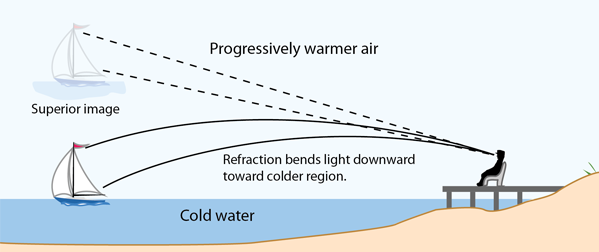
\includegraphics[width=0.95\hsize]{miragesup.png}\end{center}
A superior image can be produced when warm air exists over cold water. Again, using the pattern from Greenler, the vertical scale and the curvature are greatly exaggerated to show the effect. Such images are often seen at great distances in the arctic region when the air is significantly warmer than the water. Since the geometry of the mirage images depends on the details of the temperature contour, a great variety of mirage images can be formed.

Source: \url{http://hyperphysics.phy-astr.gsu.edu/hbase/atmos/mirage.html}
\end{block}

\vfill

\begin{block}{\refname}
\renewcommand*{\bibfont}{\small}
\addtolength{\bibitemsep}{-0.5ex}
\setlength{\biblabelsep}{0.25em}
\printbibliography[heading=none]
\end{block}

\end{frame}
\end{document}
